%%%%%%%%%%%%%%%%%%%%%%%%%%%%%%%%%%%%%%%%%%%%%%%%%%%%%%%%%%%%%%%%%%%%%%%%%
%% LaTeX book template                                                 %%
%% Author:  Amber Jain (https://github.com/amberj/latex-book-template) %%
%% License: ISC license                                                %%
%%%%%%%%%%%%%%%%%%%%%%%%%%%%%%%%%%%%%%%%%%%%%%%%%%%%%%%%%%%%%%%%%%%%%%%%%

\documentclass[a4paper,11pt,oneside]{book}
\usepackage[portuguese]{babel}
\usepackage[T1]{fontenc}
\usepackage[utf8]{inputenc}
\usepackage{lmodern}
\usepackage{hyperref}
\usepackage{graphicx} % to set a images directory
\usepackage{xcolor} % changing colors
\usepackage[hang,flushmargin]{footmisc} % remove footnote's indentation
\usepackage{amsmath} % alguns símbolos matemáticos
\usepackage{float}
% \usepackage{circuitikz} % para desenhar circuitos lógicos
\usepackage{fancyvrb} % indentation in verbatim (muito bom!)

\DeclareUnicodeCharacter{0301}{\'{e}}

\graphicspath{{./images/}} % set an default images folder

% dark theme no pdf
\pagecolor[rgb]{0.7,0.7,0.7}
%\color[rgb]{0.9,0.9,0.9} % gray

% tirando indentation dos paragraphs
\setlength{\parindent}{0ex}

%%%%%%%%%%%%%%%%%%%%%%%%%%%%%%%%%%%%%%%%%%%%%%%%%%%
% First page of book which contains 'stuff' like: %
%  - Book title, subtitle                         %
%  - Book author name                             %
%%%%%%%%%%%%%%%%%%%%%%%%%%%%%%%%%%%%%%%%%%%%%%%%%%%

% Book's title and subtitle
\title{
	\Huge \textbf{Meus Estudos em Análise e Desenvolvimento de Sistemas}  \\
	\huge PUC-MG
}

% Author
\author{
	\textsc{Bruno de M. Ruas}
}

\begin{document}

\frontmatter

\maketitle

%%%%%%%%%%%%%%%%%%%%%%%%%%%%%%%%%%%%%%%%%%%%%%%%%%%%%%%%%%%%%%%%%%%%%%%%
% Auto-generated table of contents, list of figures and list of tables %
%%%%%%%%%%%%%%%%%%%%%%%%%%%%%%%%%%%%%%%%%%%%%%%%%%%%%%%%%%%%%%%%%%%%%%%%
\tableofcontents
%\listoffigures
%\listoftables

\mainmatter

%%%%%%%%%%%%%%%%%%%%%%%%%%%%%%%%%%%%%%%%%%%%%%%%%%%%%%%%%%%%%%%%%%%%%%%%
\part{Implementação de Sistemas de Software}
%%%%%%%%%%%%%%%%%%%%%%%%%%%%%%%%%%%%%%%%%%%%%%%%%%%%%%%%%%%%%%%%%%%%%%%%

%%%%%%%%%%%%%%%%%%%%%%%%%%%%%%%%%%%%%%%%%%%%%%%%%%%%%%%%%%%%%%%%%%%%%%%%
\chapter{Projeto: Desenvolvimento Web Front-End}
%%%%%%%%%%%%%%%%%%%%%%%%%%%%%%%%%%%%%%%%%%%%%%%%%%%%%%%%%%%%%%%%%%%%%%%%

\section{Etapa 1}

Objetivo da Etapa: Definir o problema a ser solucionado e os componentes do seu grupo de trabalho. Nesta etapa você entregará como tarefa dois artefatos: a \textbf{documentação de contexto} e a \textbf{especificação do projeto}.
\\~\\
O template da documentação do projeto pode ser baixado nesse \href{https://pucminas.instructure.com/courses/87866/files/5289771?wrap=1}{LINK}
\\~\\
Microfundamentos a serem estudados:
\begin{itemize}
	\item Matemática Básica
	\item Pensamento Computacional
	\item Fundamentos de Engenharia de Software
\end{itemize}

\section{Etapa 2}

Objetivo da Etapa: Projetar a interface da aplicação e a arquitetura da solução, além de definir o ambiente de trabalho que será utilizado pela equipe para desenvolver o projeto. Os artefatos a serem produzidos são: \textbf{Projeto de Interface}, \textbf{Metodologia} e \textbf{Arquitetura da Solução}.
\\~\\
Microfundamentos a serem estudados:
\begin{itemize}
	\item Fundamentos de Engenharia de Software
	\item Desenvolvimento Web Front-End
	\item Lógica Computacional
\end{itemize}

\section{Etapa 3}

Objetivo da Etapa: Desenvolver a homepage e, pelo menos, uma funcionalidade da solução projetada. O primeiro artefato a ser gerado é o \textbf{Template do site}, que determina o layout padrão do site (HTML e CSS) que será utilizado em todas as páginas com a definição de identidade visual, aspectos de responsividade e iconografia. No desenvolvimento das funcionalidades, cada artefato gerado (código fonte) deve estar relacionado a um requisito funcional e/ou não funcional.
\\~\\
Microfundamentos a serem estudados:
\begin{itemize}
	\item Desenvolvimento Web Front-End
	\item Algoritmos e Lógica de Programação
\end{itemize}

\section{Etapa 4}

Objetivo da Etapa: Finalizar o desenvolvimento da solução e irá elaborar e executar o plano de testes funcionais. Os artefatos serão: O \textbf{plano de testes de software} e O \textbf{Registro de Testes de Software}.
\\~\\
Microfundamentos a serem estudados:
\begin{itemize}
	\item Algoritmos e Lógica de Programação
	\item Fundamentos de Engenharia de Software
	\item Algoritmos e Abstração de Dados
\end{itemize}

\section{Etapa 5}

Objetivo da Etapa: Apresentar a versão final da solução implantada.
\\~\\
A apresentação do projeto consiste na geração de um conjunto de slides em um arquivo no formato ppt, pptx ou pdf, contemplando os seguintes itens:
\begin{itemize}
	\item	Contexto (Problema, Público-alvo);
	\item	Requisitos;
	\item	Solução Implementada (funcionalidades de software);
	\item	Conclusão da elaboração do projeto (pontos positivos, desafios, aprendizado).
\end{itemize}

Recomenda-se não ultrapassar 10 slides, pois o tempo de apresentação é limitado a 10 minutos, sendo 5 minutos para o projeto (slides) e 5 minutos para a demonstração da aplicação.
\\~\\
A equipe também deverá gravar um vídeo de, no máximo, três minutos, com a apresentação da solução. Vocês deverão abrir a aplicação hospedada e apresentar o seu funcionamento.
\\~\\
Microfundamentos a serem estudados:
\begin{itemize}
	\item Fundamentos de Engenharia de Software
	\item Organização de Computadores
\end{itemize}

%%%%%%%%%%%%%%%%%%%%%%%%%%%%%%%%%%%%%%%%%%%%%%%%%%%%%%%%%%%%%%%%%%%%%%%%
\chapter{Algoritmos e Abstração de Dados}
%%%%%%%%%%%%%%%%%%%%%%%%%%%%%%%%%%%%%%%%%%%%%%%%%%%%%%%%%%%%%%%%%%%%%%%%

\section{Bibliografia}

Bibliografia Básica

\begin{itemize}
	\item ASCENCIO, Ana Fernanda Gomes; CAMPOS, Edilene Aparecida Veneruchi de. Fundamentos da programação de computadores. São Paulo: Pearson, 2012. ISBN 9788564574168
	\item SOUZA, Marco A. Furlan de; GOMES, Marcelo Marques; SOARES, Marcio Vieira; CONCÍLIO, Ricardo. Algoritmos e lógica de programação: um texto introdutório para a engenharia. São Paulo: Cengage Learning, 2019. ISBN: 9788522128150
	\item ACM TRANSACTIONS ON PROGRAMMING LANGUAGES AND SYSTEMS. New York: Association for Computing Machinery.,1979-. 6 times a year. Absorvido ACM letters on programming languages and systems. ISSN 0164-0925. Disponível em: https://dl-acm-org.ez93.periodicos.capes.gov.br/citation.cfm?id=J783
	\item AGUILAR, Luis Joyanes. Fundamentos de programação algoritmos, estruturas de dados e objetos. 3. ed. Porto Alegre: AMGH, 2008. ISBN: 9788580550146
\end{itemize}

Bibliografia Complementar

\begin{itemize}
	\item DEITEL, Harvey M; DEITEL, Paul J. Java - como programar. 8. ed. São Paulo: Pearson, 2010. ISBN 9788576055631
	\item GRIFFITHS, Ian. Programming C\# 8.0. O'Reilly Media, Inc. 2019. ISBN 9781492056812
	\item MANZANO, José Augusto N. G; OLIVEIRA, Jayr Figueiredo de. Algoritmos: lógica para desenvolvimento de programação de computadores. 28. ed. rev. e atual. São Paulo, SP: Érica, 2016. E-book. ISBN 9788536518657
	\item PROGRAMMING AND COMPUTER SOFTWARE. New York, Consultants Bureau, 1975-. Bimestral. ISSN 1608-3261. Disponível em: https://link-springer-com.ez93.periodicos.capes.gov.br/ \\ journal/volumesAndIssues/11086
	\item PRICE, Mark J. C\# 8.0 and .NET Core 3.0 - Modern Cross - Platform Development. O'Reilly Media; 2019. ISBN 9781788478120
	\item PUGA, Sandra; RISSETTI, Gerson. Lógica de programação e estruturas de dados com aplicações em Java. 2. ed. São Paulo: Prentice Hall, 2009. ISBN 9788576052074
\end{itemize}

\section{Estrutura de Dados Homogêneas e Heterogêneas}
\subsection{Estrutura de Dados Homogêneas}
\subsection{Estrutura de Dados Heterogêneas}

\section{Tipos Abstratos de Dados - Classes - Implementação}
\subsection{Definição de um TAD - Classes e Objetos}
\subsection{Atributos, Propriedades e Métodos de Classe}
\subsection{Mecanismos de Visibilidade/Acessibilidade}
\subsection{Construtores de Classe}

%%%%%%%%%%%%%%%%%%%%%%%%%%%%%%%%%%%%%%%%%%%%%%%%%%%%%%%%%%%%%%%%%%%%%%%%
\chapter{Algoritmos e Lógica de Programação}
%%%%%%%%%%%%%%%%%%%%%%%%%%%%%%%%%%%%%%%%%%%%%%%%%%%%%%%%%%%%%%%%%%%%%%%%

\section{Bibliografia}

Bibliografia Básica

\begin{itemize}
	\item Ana Fernanda Gomes ASCENCIO; Edilene Aparecida Veneruchi de CAMPOS. Fundamentos da Programação de Computadores: algoritmos, Pascal, C/C++ e Java - 2ª edição. São Paulo, SP : Pearson Education do Brasil, 2012
\end{itemize}

Bibliografia Complementar

\begin{itemize}
	\item H. DEITEL et. Al.  C\#: Como Programar. São Paulo: Makron Books, 2003
	\item John SHARP. Microsoft Visual C\# 2013. Grupo A, 2014
	\item André Luiz Villar FORBELLONE, Henri Frederico EBERSPÄCHER. Lógica de programação: a construção de algoritmos e estruturas de dados. São Paulo: Prentice Hall, 2005.
	\item MANZANO, José Augusto N. G; OLIVEIRA, Jayr Figueiredo de. Algoritmos: lógica para desenvolvimento de programação de computadores 28. ed. rev. e atual. São Paulo, SP: Érica, 2016
	\item Sandra PUGA, Gerson RISSETTI. Lógica de Programação e Estrutura de Dados: com aplicações em Java - 2ª edição. São Paulo : Pearson, 2017
\end{itemize}

\section{Lógica de Programação e Estrutura de Controle, Funções e Procedimentos}
\subsection{Conceito de Algoritmo}
\subsection{Variáveis}
\subsection{Estrutura Sequencial}
\subsubsection{Etapas de um Algotimo e o Operador de Atribuição}
\subsubsection{Operadores e Funções Aritméticas}
\subsubsection{Expressões Aritméticas}
\subsection{Estrutura Condicional}
\subsubsection{Condição Simples e Composta}
\subsubsection{Operadores Booleanes e Exemplos de Uso do Comando IF}
\subsubsection{O Comando Switch e o Operador Ternário}
\section{Estrutura de Repetição}
\subsubsection{Os Comandos WHILE, DO WHILE e FOR}
\subsubsection{Contadores e Acumuladores}

\section{Manipulação de Dados em Memória Primária e Secundária}
\subsection{Criando e Usando Funções e Procedimentos}
\subsection{Passagem de Parâmetros}
\subsection{Manipulação de Arquivos em C\#}

%%%%%%%%%%%%%%%%%%%%%%%%%%%%%%%%%%%%%%%%%%%%%%%%%%%%%%%%%%%%%%%%%%%%%%%%
\chapter{Desenvolvimento Web Front-End}
%%%%%%%%%%%%%%%%%%%%%%%%%%%%%%%%%%%%%%%%%%%%%%%%%%%%%%%%%%%%%%%%%%%%%%%%

\section{Bibliografia}

Bibliografia Básica

\begin{itemize}
	\item SIKOS, L. Web Standards. Mastering HTML5, CSS3, and XML.
	\item DACONTA, M. C.; SMITH, K. T.; OBRST, L. J. The semantic Web: a guide to the future of XML, Web services, and knowledge management. [s. l.]: Wiley, [s. d.]. ISBN 0471432571
	\item SILVA, Maurício Samy. HTML 5: a linguagem de marcação quer revolucionar a web. 2. ed. rev. e ampl. [s. l.]: Novatec, 2014. ISBN 9788575224038
	\item SANDERS, William B. Smashing HTML5: técnicas para a nova geração da web. Porto Alegre: Bookman, 2012. xiv, 354 p. ISBN 9788577809608
	\item DEITEL, Paul J., Deitel, Harvey M. Ajax, Rich. Internet Applications e Desenvolvimento Web para Programadores. Pearson 776. ISBN 9788576051619
	\item SILVA, Maurício Samy. CSS3: desenvolva aplicações web profissionais com uso dos poderosos recursos de estilização das CSS3. São Paulo: Novatec, 2011. 494 p. ISBN 9788575222898
	\item BERTAGNOLLI, S. de C.; MILETTO, E. M. Desenvolvimento de software II: introdução ao desenvolvimento web com HTML, CSS, JavaScript e PHP. [s. l.]: Bookman, 2014. ISBN 9788582601952
\end{itemize}

\section{A Web: Evolução, Padrões e Arquitetura}
\subsection{Histórico e Evolução da Web}

A Web é um sistema da informação de hipertextos onde o acesso é feito por meio de \textbf{navegadores (browsers)}.
\\~\\
Existem alguns protocolos comuns para transferência de alguns tipos de arquivos. Para mensagens (e-mail) usamos o \textbf{SMTP}, para transferência de arquivos usamos o \textbf{FTP}, aplicações de telefonia usam o \textbf{VOIP} e para páginas de conteúdo usamos o \textbf{HTML}.
\\~\\
A história da web eu ainda vou colocar aqui quando tiver mais tempo.

\subsection{W3C e os Padrões da Web}

O WORLD WIDE WEB CONSORTIUM (W3C) é uma organização sem fins lucrativos cujo lider é o Tim Berners-Lee, justamente o inventor da Web. Existem várias ogranizações ao longo do planeta que fazem parte desse consórcio internacional.

O W3C mantém a gestão de vários padrões usados todos os dias:
\begin{itemize}
	\item Design e Aplicações Web (HTML, CSS, SVG, Ajax, Acessibilidade);
	\item Arquitetura da Web (Protocolo HTTP, URI);
	\item Web Semântica (Linked Data - RDF, OWL, SPARQL);
	\item Web Services (SOAP, WSDL);
	\item Tecnologia XML (XML, XML Schema, XSLT);
	\item Navegadores e ferramentas de autoria.
\end{itemize}

A W3C possui um processo de publicação das normativas. Normalmente, o fluxo é:
\begin{itemize}
	\item Working Draft (WD)
	\item Candidate Release (CR)
	\item Proposed Recomendation (PR)
	\item Recomendation (REC)
\end{itemize}

\subsection{Componentes da Arquitetura da Web}

A web pode ser entendida como uma coleção de componentes que permitem a comunicação entre o cliente e os servidores de aplicações. Os principais componentes dessa arquitetura são:
\begin{itemize}
	\item Ambiente Cliente (Client Web) \\~\\
			Geralmente um Browser que envia as requisições usando o protocolo HTTP(S) para o servidor web através de uma rede de computadores.
	\item Ambiente Servidor \\~\\
			O ambiente servidor possui vários componentes (banco de dados, aplicações, API e etc) mas o principal componente é o servidor web. Ele recebe a requisição HTTP(S) do client, interpreta a URL e envia os recursos solicitados (HTML, CSS, JS, JPEG, MP4 e etc) por meio da rede. 
	\item Internet \\~\\
			É a rede mundial baseada no protocolo TCP/IP onde todo computador conectado é denominado host (hospedeiro) e possui um identificador de endereço IP (internet protocol) que possui determinados padrões.
	\item URI (uniform resource locator) \\~\\
			Como o nome indica, um URI é um localizado que pode ser classificado em duas maneiras. O URL é o tipo de URI que usa o endereço do conteúdo como método de localização, ele nos diz onde encontrar o recurso (por exemplo, o caminho \verb|c://home/desktop/test.txt|). O URN é o tipo que usa o nome do recurso, ele nos diz a identidade do item procurado (por exemplo, o sistema ISBN). 
	\item Requisição \\~\\
			É o pacote de dados enviado pelo client através da internet para o web server onde está a instrução do que deve ser enviado como resposta.
	\item Resposta \\~\\
			Como o nome já diz, é o retorno do web server ao client com os dados requisitados.
	\item Protocolo HTTP \\~\\
			É o padrão como client e web server se comunicam pela rede.
\end{itemize}

\subsection{URI, URL e URN}

Já vimos que o URI abarca dos conceitos de URL e URN. Agora vamos aprender um pouco mais sobre os padrões de endereços em ambos os protocolos.

\subsubsection{URL}

O padrão URL serve para identificar o recurso pela sua localização e é composto da seguinte maneira:

\begin{center}
	\verb|ftp://example.com:8080/pasta/arquivo?name=book#nose| \\
	Cujas partes são \\
	\verb|scheme://authority/path?query#fragment|
\end{center}

Como podemos ver, a URL é composta por várias partes:
\begin{itemize}
	\item scheme - é a forma de interação (ftp, http, https, ...).
	\item user:pass - são as informações do user.
	\item host - endereço de ip do server.
	\item porta - qual a porta TCP/IP do server (o padrão http é 80 e pode ser omitida).
	\item path - local onde o recurso se encontra.
	\item query - detalhe da consulta na forma de pares nome-valor.
	\item fragmento - qual seção do recurso.
\end{itemize}

\subsubsection{URN}

\begin{center}
	\verb|urn:example:animal:ferret:nose| \\
	Cujas partes são \\
	\verb|scheme:path:authority|
\end{center}

A URN apenas nos dá um recurso específico (NSS) contido em algum namespace (NID) sem qualquer informação sobre onde o arquivo está localizado.

\subsection{Protocolo HTTP}

O hypertext transfer protocol é mantido pela W3C e rege a camada de aplicação dos sistemas distribuídos de informação em hipertexto. Existem muitas versões mas a mais utilizada é a 2.0 de 2015.
\\~\\
Para entender melhor o http, consideremos o processo usual de navegação na web:
\begin{enumerate}
	\item user informa a URL
	\item client monta a requisição http e envia ao web server
	\item server recebe a requisição e envia a resposta ao client
	\item a resposta é recebida e interpretada pelo browser com os dados exibidos ao user
	\item dependendo da página, pode ser que novas requisições sejam feitas para que todos os componentes sejam carregados propriamente.
\end{enumerate}

Podemos ver que o http é o conjunto de regras que rege a comunicação client-server da web.

\subsubsection{Partes da requisição HTTP}

Uma requisição é formada por 3 partes:
\begin{itemize}
	\item Linha de Requisição
		\begin{itemize}
			\item Método
				\begin{itemize}
					\item GET - Requisita dados.
					\item POST - Envia dados para o server.
					\item HEAD - Requisita dados mas o retorno deve ser um conjunto de cabeçalhos.
					\item PUT - Criação ou Atualização de dados.
					\item DELETE - Excluir algum dado.
					\item TRACE - Solicita uma cópia da requisição (serve pra testar integridade).
					\item PATCH - Alterações parciais em um recurso.
					\item OPTIONS - Lista de métodos e opções disponíveis para o server.
					\item CONNECT - Usado quando o client se conecta com o server via proxy.
				\end{itemize}
			\item Recurso - É o caminho do dado requerido.
			\item Versão do Protocolo - Qual versão do http será usada.
		\end{itemize}
	\item Linhas de Cabeçalho \\
			Inclui informações complementares à requisição sendo formado por pares nome-valor.
	\item Corpo da Entidade \\
			Dados adicionais como forms, arquivos para upload e etc.
\end{itemize}

\subsubsection{Partes da resposta HTTP}

\begin{itemize}
	\item Linha de Resposta
		\begin{itemize}
			\item Versão HTTP.
			\item Código de Retorno.
			\item Mensagem explicativa do código de retorno.
		\end{itemize}
	\item Linhas de Cabeçalho \\
			Uma informação importante que consta no cabeçalho é o \verb|content-type|. Ele diz o formato do conteúdo enviado como resposta\footnote{Isso pode ser a causa de alguns bugs na sua aplicação.}. Essa informação é apresentada conforme os \href{https://developer.mozilla.org/pt-BR/docs/Web/HTTP/Basics_of_HTTP/MIME_types}{MIME Types}.
	\item Corpo da Entidade
			É o recurso solicitado pelo client (html, css, js, jpeg, mp4, ...)
\end{itemize}

\subsubsection{Um pouco mais sobre Cabeçalhos}

Os cabeçalhos possuem características parecidas tanto nas requests quanto nas responses. Podemos classifica-los como sendo dos tipos:
\begin{itemize}
	\item Request header - Informações sobre o client ou a requisição feita.
	\item Response header - Informações sobre a resposta ou sobre o web server.
	\item Entity header - Informações sobre o conteúdo da entidade trocada (tamanho e tipo).
	\item General header - Informações gerais usadas tanto em requests quanto em responses.
\end{itemize}

\subsection{Servidores Web}

Você só consegue visualizar as informações de um site porque o servidor web foi capaz de interpretar a requisição feita pelo seu browser e responder com o conteúdo adequado. Agora vamos entender um pouco mais sobre o ambiente servidor.
\\~\\
O principal elemento do ambiente servidor é o web server. Ele é quem recebe, interpreta e responde as requisições dos clients ao longo da internet. Podemos também incluir outros elementos importantes no ambiente servidor como o \textbf{servidor de banco de dados} e os \textbf{servidores de serviços (APIs)}.

\begin{figure}[H]
	\centering
	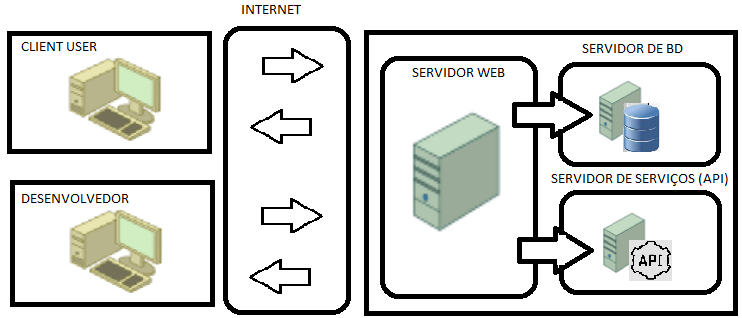
\includegraphics[scale=0.6]{08-arq_web.png}
	\caption{Esboço da arquitetura web}
\end{figure}

\subsubsection{Funções de um web service}

Um web server nada mais é que um software rodando em uma máquina. Ele desempenha várias funções que podemos elencar como:
\begin{itemize}
	\item Atender as requests http e responder a elas.
	\item Gerencias sites.
	\item Gerencias arquivos dos sites.
	\item Integrar mecanismos de scripts: php, perl, aspx, Ruby, Python e etc.
	\item Autenticar users (básica ou com servidores de autenticação).
	\item Implementar criptografia nas comunicações (https - tls/ssl).
	\item Cache de recursos.
	\item Auditoria das alterações e logs.
\end{itemize}

\subsubsection{Software e Provedores}

Basicamente, existem 3 formas de tornar uma aplicação web acessível aos clients: Rodar um web server na máquina local; instalar e configurar um wer server em uma máquina dedicada para esse trabalho e, por fim, contratar um provedor que ofereça esse serviço.
\\~\\
A lista de softwares que se propõe a fazer o trabalho de um web server é enorme. O material do curso elenca dois:
\begin{itemize}
	\item Apache HTTP Server | \href{https://httpd.apache.org/}{Apache Web Server} \\
			É um open source multi plataforma. Permite execução de multilinguagens como php, perl entre outras. Uma maneira simples de instalar é pelo \href{https://www.apachefriends.org/index.html}{XAMPP} (que já integra o apache web server, banco de dados MariaDB e um ambiente PHP e Perl).
	\item Microsoft Internet Information Server (IIS) \\
			É a solução proprietária da Microsoft. Baseado na plataforma .NET, permite hospedar sites estáticos. O IIS já vem disponível junto dos SO Windows.
\end{itemize}

A lista de provedores também é extensa  e possuem diferentes capacidades distintas mas podemos destacar algumas ferramentas úteis:
\begin{itemize}
	\item Servidores em Nuvem
	\begin{itemize}
		\item \href{https://azure.microsoft.com/pt-br/}{Azure}
		\item \href{https://www.heroku.com/}{Heroku}\footnote{Esse aqui eu to estudando e fazendo um manual de como usar. Você pode ler o manual nesse \href{https://github.com/brunoruas2/Analise_Des_Sistemas/tree/main/Manuals/heroku}{[LINK]}}
		\item \href{https://aws.amazon.com/pt/}{AWS}
	\end{itemize}

	\item Editores e IDEs online
	\begin{itemize}
		\item \href{https://replit.com/}{Replit}
		\item \href{https://codesandbox.io/}{CodeSandbox}
		\item \href{https://glitch.com/}{Glitch}
		\item \href{https://pages.github.com/}{GitHub Pages}
	\end{itemize}
\end{itemize}

\subsection{Dinâmica de Aplicações Web}

Quando você acessa um site, o arquivo que coordena o modo de exposição da informação e os conteúdos da mesma é um arquivo ``\verb|.html|''. Observe o exemplo abaixo de uma página simples.

\begin{Verbatim}[tabsize=4,frame=single]
<!DOCTYPE html>
<html lang="en">
	<head>
		<meta charset="UTF-8">
		<title>Document</title>
		<link rel="stylesheet" href="style.css">
		<script> src='app.js'</script>
	</head>
	<body>
		<img src='logo.jpg' alt="imagem_logo">
	</body>
</html>
\end{Verbatim}

As tags que contém as partes \verb|style.css|, \verb|app.js| e \verb|logo.jpg| fazem menção à outros arquivos que farão parte da composição da página. Alguns são referentes à funcionalidades ou layout da aplicação enquanto outros podem ser referentes à conteúdos mostrados na página.
\\~\\
Uma vez que o servidor compreende a request feita pelo client, ele envia uma série de arquivos que serão lidos pelo browser do usuário e serão interpretados por ele. O html é justamente o primeiro arquivo lido porque ele diz ao navegador quais conteúdos mostrar e, a partir das referências contidas no html, como mostrar e quais funcionalidades a página terá.

\subsubsection{O processamento de um site}

\begin{enumerate}
	\item O client envia uma requisição via http (com o método GET) para o web server
	\item O server envia o arquivo html da página requisitada para o browser
	\item Ao processar o html, o browser percebe que ele faz menção de outros arquivos (como css, js, mp3, etc)
	\item O browser faz novas requisições ao server até ter todos os arquivos necessários para o carregamento da página
\end{enumerate}

Como você pode ver, é muita coisa acontecendo. Só não nos damos conta disso porque o processo é muito rápido hoje em dia devida a velocidade das nossas conexões banda larga. Lembrando sempre que todas as requisições e respostas entre client e server são feitas usando-se o protocolo HTTP que a gente viu logo antes.

\section{Desenvolvimento de Interfaces Web}

\subsection{A Linguagem HTML}

A linguagem HTML foi criada por Tim Berners-Lee no ano de 1991 e foi baseada no padrão Standard Generalized Markup Language (SGML). Seu escopo original era para permitir a divulgação de pesquisas científicas.
\\~\\
Com o passar dos anos, novas tecnologias foram somadas ao ecossistema para facilitar o processo de construção das soluções web. O Cascading Style Sheet (CSS) foi criado para facilitar o desenvolvimento do conteúdo separando a parte de estilo e aparência do conteúdo em HTML. O JavaScript permitiu a manipulação de elementos além de dar mais dinâmica para as páginas web.
\\~\\
O W3C foi criado em 1993 e, a partir dessa data, o HTML foi mantido e padronizado por essa organização. Desde então a linguagem vem sendo alterada para permitir sua evolução.
\\~\\
Em 2004 foi criado o Web Hypertext Application Technology Working Group (WHATWG) por pessoas da Apple, Mozilla e Opera. Na época, o W3C estava trabalhando no padrão XHTML 2.0 (que iria substituir o HTML 4.01) mas o WHATWG conseguiu propor um monde que acabou sendo o HTML 5. O HTML 5 foi recebido e amplamente adotado no desenvolvimento de aplicações hoje em dia.
\\~\\
\textbf{Panorama de uma Aplicação}
\\~\\
Nós já sabemos que um client faz uma requisição ao web server por HTTP e esse, por sua vez, responde a requisição com, normalmente, um arquivo HTML. De posse de arquivo, o browser consegue saber se precisará solicitar mais arquivos ao web server até que todas as referências do HTML sejam satisfeitas e a página carregada.
\\~\\
A grosso modo, podemos dizer que o HTML pode fazer menções a arquivos dos seguintes tipos:
\begin{itemize}
	\item CSS
	\item Arquivos de Multimídia
	\item JavaScript
	\item RIA - Rich Internet Applications
		\begin{itemize}
			\item Applet Java
			\item Adobe Flash
			\item Adobe Air
			\item Adobe Flex
			\item SilverLight
		\end{itemize}
\end{itemize}

Se o site utiliza soluções dinâmicas como PHP, Java, Python, Ruby ou ASP.NET, quando a requisição é feita, o web server primeiro faz o processamento desses arquivos (normalmente por um outro servidor de APIs) e o resultado serão outros arquivos HTML, CSS, JS ou Multimídia. Após o processamento, o resultado é enviado para o client que será atualizado pelo browser.
\\~\\
Nas aplicações modernas, o seu browser está em processo praticamente contínuo de interação com o servidor e vice-versa.
\\~\\
\textbf{A Sintaxe da Linguagem HTML}
\\~\\
Uma página HTML é uma coleção de \textbf{elementos}. Você consegue identificá-los facilmente porque estão entre os pares de símbolos \verb|<>|. Cada elemento também tem uma tag de abertura e uma de fechamento. Por exemplo:

\begin{center}
	\verb|<body> Aqui vai o conteúdo do body </body>|
\end{center}

Também existem elementos que não precisam do par de tags de abertura e fechamento. Por exemplo:

\begin{center}
	\verb| <input disable name='Nome' value='rommelcarneiro'>|
\end{center}

Atente para o fato que alguns elementos aceitam outros elementos internamente. Por exemplo, dentro do elemento \verb|<body></body>| nós colocamos todos os outros elementos que comporão a nossa página web, como por exemplo, formulários, parágrafos, vídeos e etc. Então se acostume de termos elementos dentro de outros elementos.
\\~\\
Dentro de alguns elementos podem ser inseridas informações e configurações por meio de parâmetros que chamamos de \textbf{atributos} do elemento. Por exemplo, no elemento logo acima, temos os atributos \verb|name| e \verb|value|.
\\~\\
Agora que sabemos o que são elementos e como eles são construídos, podemos seguir para a \textbf{organização de um documento HTML}. Existe um padrão em todo arquivo HTML onde existem alguns elementos obrigatórios para o processamento da página pelo browser do client.

\begin{Verbatim}[tabsize=4,frame=single]
<!DOCTYPE html> -----------------> Elemento da versão do HTML
<html lang="en"> ----------------> Abertura do documento HTML 
	<head> ----------------------> Abertura do cabeçalho      
		<meta charset="UTF-8"> --> Atributo nome = "valor"    
		<title>Document</title> -> Elemento de Título         
	</head> ---------------------> Fechamento do cabeçalho
	<body> ----------------------> Abertura do corpo
		<img src="logo.jpg"> ----> Elemento de imagem         
	</body> ---------------------> Abertura do corpo
</html> -------------------------> Fechamento do HTML
\end{Verbatim}

\textbf{Preâmbulo}
\\~\\
Como podemos ver, primeiro temos o preâmbulo \verb|DOCTYPE|, seguido do \verb|<html> </html>| onde temos outros dois elementos maiores, o cabeçalho (\verb|<head> </head>|) e o corpo (\verb|<body> </body>|).
\\~\\
O preâmbulo diz ao navegador qual versão da HTML será usada. Se ele não for indicado, o navegador vai tentar ``adivinhar'' qual a melhor maneira de interpretar a sua página (chamamos isso de \textbf{quirks mode}). Caso você informe qual a versão, o browser usará o processamento adequado (chamamos de \textbf{strict mode}). Os formatos do preâmbulo mudam de acordo com a versão do HTML:
\begin{itemize}
	\item HTML 5
		\verb|<!DOCTYPE html>|
	\item HTML 4.01
	\verb|<!DOCTYPE HTML PUBLIC "-//W3C//DTD HTML 4.01 Transitional//EN"|
	\verb|"http://www.w3.org/TR/html4/loose.dtd">|
	\item HTML 1.0
	\verb|<!DOCTYPE html PUBLIC "-//W3C//DTD XHTML 1.0 Transitional//EN"| 
	\verb|"http://www.w3.org/TR/xhtml1/DTD/xhtml1-transitional.dtd">|
\end{itemize}

\textbf{Cabeçalho}
\\~\\
É a primeira parte dentro da tag de html. Nele estão as informações sobre o documento de modo a organizar as referências de funcionalidade que serão usadas para o processamento da página web. Podemos resumir os elementos no cabeçalho como:
\begin{itemize}
	\item title - \verb|<title> </title>| \\
		Define o título do documento. Que também afeta a aba do navegador.
	\item link - \verb|<link rel="relacao" href="link_do_arquivo.extensao">| \\
		Define as ligações externas como arquivos, scripts, CSS e etc. 
	\item style - \verb|<link rel="stylesheet" href="style.css">| \\
		É um tipo de link. Nele é que vamos indicar qual o arquivo que regerá o layout da nossa aplicação.
	\item meta - \verb|meta name="nome" content="conteudo">| \\
		Aqui teremos as informações adicionais sobre a página: codificação de caracteres, descrição, palavras-chaves, autor e etc.
\end{itemize}

\textbf{Corpo}
\\~\\
A segunda parte do html é o corpo. Nele é onde colocamos o conteúdo que fará parte da página. Como é muito comum de se encontrar nos sites, esse conteúdo pode vir mesclado em várias mídias como texto, imagens, vídeos, mapas e etc. Veremos com calma um pouco mais a frente.

\subsubsection{Elementos de Texto e Multimídia}

Como esse material tem o objetivo de ser para futuras consultas. Eu vou colocar as tags com um pequeno resumo mas não vou comentar muito sobre elas.
\\~\\
\textbf{Parágrafos e Títulos}

\begin{center}
	\begin{tabular}{|c|c|}
		\hline
		\textbf{Elemento} & \textbf{Tags} \\
		\hline
		Títulos & \verb|<h1></h1>,...,<h6></h6>| \\
		\hline
		Parágrafo & \verb|<p></p>| \\
		\hline
		Quebra de Linha & \verb|<br>| \\
		\hline
		Itálico & \verb|<i></i>| \\
		\hline
		Negrito & \verb|<b></b>| \\
		\hline
		Importância & \verb|<strong></strong>| \\
		\hline
		Código-fonte & \verb|<code></code>| \\
		\hline
		Texto pre-formatado & \verb|<pre></pre>| \\
		\hline
		Citações & \verb|<blockquote></blockquote>| \\
		\hline
	\end{tabular}
\end{center}

Enquanto estamos montando a nossa página html, devemos evitar usar os elementos dela para a formatação de layout da nossa solução. É altamente recomendado deixar toda essa responsabilidade para a nossa Cascading Style Sheets (CSS) e focar apenas no conteúdo textual da página web.
\\~\\
\textbf{Listas}
\\~\\
Existem 3 tipos de listas em HTML.
\\~\\
Listas ordenadas:
\begin{Verbatim}[tabsize=4,frame=single]
<ol>
	<li> Primeiro item </li> --------> 1. Primeiro item
	<li> Segundo item </li> ---------> 2. Segundo item
	<li> Terceiro item </li> --------> 3. Terceiro item
</ol>
\end{Verbatim}

Lista não ordenada:
\begin{Verbatim}[tabsize=4,frame=single]
<ul>
	<li> Primeiro item </li> --------> o Primeiro item
	<li> Segundo item </li> ---------> o Segundo item
	<li> Terceiro item </li> --------> o Terceiro item
</ul>
\end{Verbatim}

Lista de definições:
\begin{Verbatim}[tabsize=4,frame=single]
<dl>
	<dt> Termo 01 </li> -------------> Termo 01
	<dd> Definição 01 </li> ---------> 		Definição 01
	<dt> Termo 02 </li> -------------> Termo 02
	<dd> Definição 02 </li> ---------> 		Definição 02
</dl>
\end{Verbatim}

\textbf{Imagens}
\begin{Verbatim}[tabsize=4]
	<img width="200" height="180" src="img.png" alt="Peixe">
\end{Verbatim}

\textbf{Links}
\begin{Verbatim}[tabsize=4]
<a href="link.com" target="_blank"> Texto </a> ------> Nova tab
<a href="link.com" target="_self"> Texto </a> -------> Mesma tab
<a href="link.com" target="_parent"> Texto </a> -----> Frame pai
<a href="link.com" target="_top"> Texto </a> --------> Janela atual
<a href="link.com" target="nome_frame"> Texto </a> --> Frame nominado
\end{Verbatim}

\subsubsection{Elementos Estruturais}

A partir da versão 4.0 o principal elemento usado para segmentar as partes de uma página html passou a ser o \verb|<div>| que é um um elemento de divisão genérico para agrupar qualquer conjunto de elementos necessários. Por exemplo:

\begin{Verbatim}[tabsize=4,frame=single]
<div>
    <h1> Titulo </h1>
    <p> Parágrafo pequeno </p>
    <ol>
        <li>Item</li>
        <li>Item</li>
    </ol>
</div>
\end{Verbatim}

Na versão 5 do HTML passamos a ter vários tipos de elementos com a mesma função dos \verb|<div>| mas agora com nomes mais fáceis de usar. As vezes nos referimos a eles como \textbf{elementos semânticos}. O novos elementos semânticos apresentados na versão 5 do html são:

\begin{center}
	\begin{tabular}{|c|c|}
		\hline
		\textbf{Elementos} & \textbf{Descrição} \\
		\hline
		\verb|<article>| & Define um artigo \\
		\hline
		\verb|<aside>| & Conteúdo ao lado da página \\
		\hline
		\verb|<details>| & Detalhes adicionais \\
		\hline
		\verb|<figcaption>| & Título para \verb|<figure>| \\
		\hline
		\verb|<figure>| & Elemento autocontido \\
		\hline
		\verb|<footer>| & Rodapé para seção \\
		\hline
		\verb|<header>| & Cabeçalho para seção \\
		\hline
		\verb|<main>| & Conteúdo principal \\
		\hline
		\verb|<mark>| & Texto destacado \\
		\hline
		\verb|<nav>| & Conteúdo de navegação \\
		\hline
		\verb|<section>| & Seção do documento \\
		\hline
		\verb|<summary>| & Resumo \\
		\hline
		\verb|<time>| & Define data/hora \\
		\hline	
	\end{tabular}	
\end{center}

Quando construímos a estrutura do nosso site apenas com elementos \verb|<div>| genéricos, nós não estamos indicando nenhuma relação entre essas seções. Quando usamos a divisão via elementos semânticos, permitimos um processamento por algoritmos de modo a abrir todo um leque de possibilidades de interações a partir disso. Esse é um dos motivos que justificam o nome da web 3.0 como sendo \textbf{web semântica}. 
\\~\\
Abaixo temos duas maneiras de representar uma estrutura de um site. A primeira em estrutura genérica de \verb|div| e a outra em elementos semânticos. Veja como a segunda abordagem é mais simples de ler.

\begin{figure}[H]
	\centering
	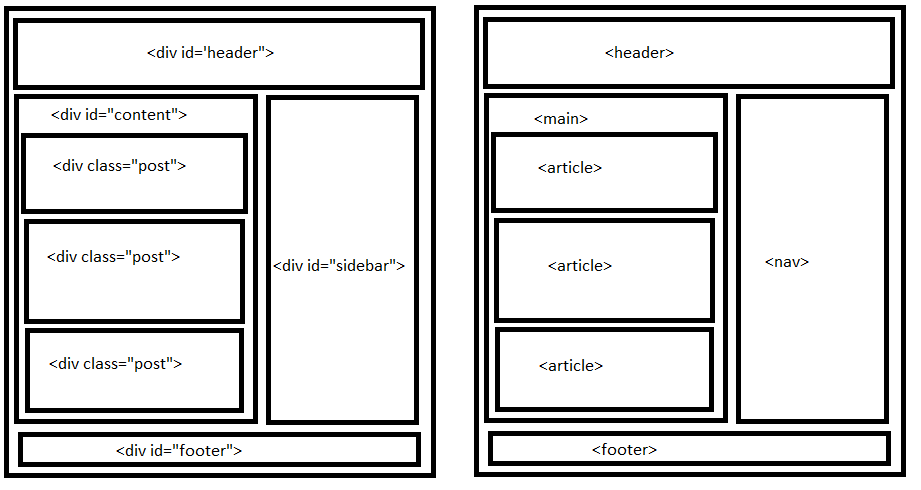
\includegraphics[scale=0.5]{09-divs_semantic.png}
	\caption{Estrutura em <div> versus Estrutura em elementos semânticos}
\end{figure}

Não é difícil perceber que o uso de elementos semânticos é fortemente indicado para o desenvolvimento de aplicações web modernas.

\subsubsection{Elementos de Tabelas}

Não é nada incomum ter que demonstrar dados usando uma tabela. Pensando nisso, a linguagem HTML também possui um elemento especificamente criado para criação de tabelas. Uma tabela pode ser criada com o uso das seguintes tags:

\begin{Verbatim}[tabsize=4,frame=single]
<table border="1"> --------------> Cria a Tabela
	<caption> Título </caption> -> Coloca um Título
	<tr> ------------------------> Table Row (tr)
		<td>L1C1</td> -----------> Table Data Column 1
		<td>L1C2</td> -----------> Table Data Column 2
	</tr>
	<tr>
		<td>L2C1</td> -----------> Table Data Column 1
		<td>L2C2</td> -----------> Table Data Column 2
	</tr>
</table>
\end{Verbatim}

Existem vários elementos que podem ser usados dentro de uma tabela. São os principais:

\begin{center}
	\begin{tabular}{|c|c|}
		\hline
		\textbf{Elementos} & \textbf{Descrição} \\
		\hline
		\verb|<table>| & Elemento que cria a tabela \\
		\hline
		\verb|<caption>| & Título da tabela \\
		\hline
		\verb|<thead>| & Linhas do cabeçalho \\
		\hline
		\verb|<tbody>| & Linhas do body \\
		\hline
		\verb|<tfoot>| & Linhas do rodapé \\
		\hline
		\verb|<tr>| & Linha da tabela \\
		\hline
		\verb|<th>| & Cabeçalho dentro de uma linha \\
		\hline
		\verb|<td>| & Table data \\
		\hline
	\end{tabular}
\end{center}

\textbf{Comentário:} Não podemos cair na tentação de usar tabelas como ferramenta de layout da página. Pode até parecer mais simples no começo mas tabelas não são boas para criação de aplicações fluidas e dinâmicas.

\subsubsection{Elementos de Formulários}

Uma das interações mais básicas que precisamos de um usuário é a inserção de dados na aplicação. Dentre as várias maneiras de conseguirmos um dado inserido pelo usuário, o formulário é a mais simples.
\\~\\
O HTML fornece vários atributos dentro do elemento \verb|<form></form>| que nos permite a criar campos de texto, botões clicáveis, campos de senha e etc. A sintaxe mais básica de um formulário é dada por:

\begin{Verbatim}[tabsize=4,frame=single]
<form name="form_name" action="login.html" method="POST">
	Usuário: <br>
	<input type="text" name="user" value=""> <br>
	Senha: <br>
	<input type="password" name="psw" value=""> <br> <br>
	<input type="submit" value="OK">
</form>
\end{Verbatim}

Podemos usar o atributo \textbf{name} ou \textbf{id} para identificar o nosso formulário\footnote{Isso é muito importante porque vamos usar essa informação para fazer alguma coisa.}. O atributo \textbf{action} indica qual URL vai ser disparada uma vez processado o form (no nosso exemplo seria algo como \verb|http://server.com/login.html|). O atributo \textbf{method} indica o método HTTP de submissão dos dados do formulário no nosso bando de dados (pode ser \verb|POST| ou \verb|GET|).
\\~\\
Quando o método usado for o \verb|GET|, o browser faz uma requisição da \verb|URL| indicada para o servidor passando os parâmetros de input como \textbf{querystring} na URL. No nosso exemplo, ficaria como \verb|http://server.com/login.html/| \verb|login.html?user=texto&psw=123|.
\\~\\
Quando o método escolhido é o \verb|POST|, os dados são enviados ao servidor no corpo da requisição HTTP e não aparecem na URL. A essa altura você já deve ser capaz de entender as diferenças entre esses dois métodos.
\\~\\
\textbf{Elemento} \verb|<input>|
\\~\\
Esse elemento é bastante utilizado na composição dos formulários (na verdade, eu nem consigo pensar em um formulário sem pelo menos um input). Ele define os campos ou entradas de informação e possui os seguintes atributos:
\begin{itemize}
	\item \verb|type| - Cada tipo de input possui uma visualização diferente quando a página é carregada. Isso é feito para permitir uma melhor interação do usuário de acordo com a natureza da informação requerida. As opções são:
		\begin{itemize}
			\item text - Campo de texto aberto. A quantidade de caracteres pode ser controlada pelo atributo \verb|maxlength|.
			\item number - Só aceita número como input e permite a seleção por umas setinhas que aparecem ao lado do campo.
			\item password - Igual ao campo texto mas com os caracteres anonimizados.
			\item email - Confere se o texto inserido possui um @ antes de salvar o formulário.
			\item date - Coloca uma máscara no formato de data e cria uma opção de input por calendário.
			\item radio button - Uma opção clicável com um valor associado e um nome. O navegador só permite que um único radio button esteja selecionado se existir mais de uma opção com o mesmo nome no atributo \verb|name|.
			\item checkbox - Mesma lógica do radio button mas com permissão de vários selecionados simultaneamente.
			\item submit - É um botão clicável que normalmente dispara a informação do formulário ao servidor web ou a um script JS local.
			\item reset - É igual um submit mas a única função dele é apagar tudo que foi preenchido no formulário.
		\end{itemize}
	\item \verb|name| - Nome de identificação do campo.
	\item \verb|value| - Valor contudo no campo.
	\item \verb|placeholder| - Valor que aparece quando o campo estiver vazio.
	\item \verb|required| - Validação automática para evitar o não preenchimento do campo antes da submissão do form.
	\item \verb|disabled| - Inativa o campo e não permite interação mas o user ainda poderá ver.
\end{itemize}

Na imagem abaixo podemos ver como cada tipo do elemento \verb|<input>| aparece para um usuário:

\begin{figure}[H]
	\centering
	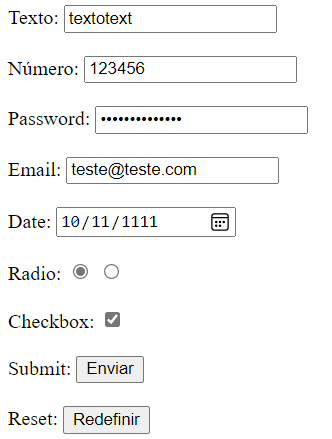
\includegraphics[scale=0.4]{10-forms.png}
	\caption{Tipos de elementos <input> dentro de um formulário html.}
\end{figure}

\textbf{Elemento} \verb|<textarea>|
\\~\\
Esse é tranquilo de entender. Sempre que precisarmos de um input de texto maior do que uma linha, podemos usar o elemento \verb|<textarea name="" rows="10"| \verb|cols="50"></textarea>| para isso. É possível alterar a quantidade de linhas e a número de colunas para apresentação da nossa caixa de texto apenas mudando os parâmetros dos atributos.
\\~\\
\textbf{Elemento} \verb|<select>|
\\~\\
Podemos permitir que o usuário selecione uma lista pré-selecionada de opções através de uma \textbf{lista em caixa} (também chamada de \textbf{dropdown menu}). Um exemplo de código contendo esse elemento por ser visto abaixo.

\begin{Verbatim}[tabsize=4,frame=single]
<label for="lista"> Dropdown Menu </label>
<select name="lista">
	<option value="">Selecione uma opção</option>
	<option value="01">Opção 01</option>
	<option value="02">Opção 02</option>
	<option value="03">Opção 03</option>
	<option value="04">Opção 04</option>
	<option value="05">Opção 05</option>
</select>	
\end{Verbatim}

É possível transformar a lista suspensa em uma lista fixa que permite mais de uma seleção. Para fazer isso é só adicionar o atributo \verb|multiple| e também o atributo \verb|size=| no elemento \verb|select|.
\\~\\
Perceba que além do elemento de lista nós trouxemos um novo elemento chamado \verb|label| que adiciona um texto associado a algum elemento. No nosso exemplo, veja como foi indicado no atributo \verb|for| o mesmo nome que o atributo \verb|name| recebe dentro do elemento \verb|select|.
\\~\\
O resultado pode ser visto abaixo:

\begin{figure}[H]
	\centering
	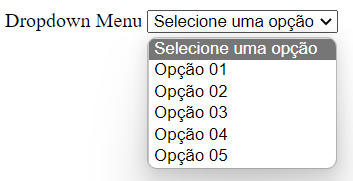
\includegraphics[scale=0.6]{11-dropdown.png}
	\caption{Tipos de elementos <input> dentro de um formulário html.}
\end{figure}

\subsection{A Linguagem CSS}

Nós falamos na parte inicial do nosso estudo sobre HTML, mas especificamente na parte do cabeçalho, que uma das referências que normalmente fazemos é a de uma \textbf{Cascading Style Sheet (CSS)}. A ideia por trás disso é que a manutenção e o desenvolvimento da aplicação web fica mais simples quando trabalhamos todo o aspecto de estilo visual em um arquivo separado (.css) do arquivo que trata da estrutura da aplicação (.html).
\\~\\
Contudo, na realidade, existem outras formas de trabalhar o visual da aplicação além do arquivo .css em separado. No geral, podemos dizer que existem 3 formas de gerenciamento de estilo de um aplicação web:
\begin{itemize}
	\item CSS externo - Melhor forma. Nosso material estará focado nesse tipo de arquitetura.
	\item Bloco interno - As regras ficam no próprio arquivo html. Pode ter aplicações para questões muito específicas. Mas as atualizações vão precisar ser feitas em cada página, sempre que necessário.
	\item Atributo inline - Pior forma. Aqui, as regras de estilo são definidas diretamente no elemento html. Qualquer mínima alteração terá de ser feita diretamente no elemento e em todas as páginas.
\end{itemize}

Aqui podemos ver um exemplo de cada aplicação do estilo visual que elencamos acima:
\begin{Verbatim}[tabsize=4,frame=single]
<!DOCTYPE html>
<html lang="en">
<head>
	<title>Exemplo CSS</title>

	###Esse é um exemplo de arquivo externo###
	<link rel="stylesheet" href="style.css" type="text/css">

	###Exemplo de bloco interno####
	<style type="text/css">
		p {
			font-size: 10pt;
			font-family: "Verdana";
			color: blue;
		  }
		
		h1 { font-size: 16pt; 
			 font-family: "Impact"; 
			 color: red;
			}
	</style>

</head>
<body>
	####Exemplo de inline#####
	<p style="margin-left: 0.5in; font-size: 8pt;">
		Texto do parágrafo
	</p>
</body>
</html>
\end{Verbatim}

A prioridade de leitura das regras de estilo que o browser vai usar é 1) inline, 2) Bloco interno, 3) CSS externo e 4) Default do navegador.
\\~\\
\textbf{Sintaxe da linguagem CSS}
\\~\\
A leitura de um arquivo CSS é bem simples. A primeira coisa que precisamos saber é quais elementos estão presentes no html que será trabalhado e quais desses elementos possuem atribuição de id específico. 
\\~\\
Por exemplo, se tivermos no nosso html dois elementos \verb|<p>|, só que um deles possui o atributo id (\verb|<p id="teste">|). Para criarmos uma regra de estilo no nosso CSS basta escrevermos a tag do elemento (sem os símbolos \verb|<>|) do seguinte modo.

\begin{Verbatim}[tabsize=4]
p {
	color: red;
}
\end{Verbatim}

Essa regra diz que todos os textos contidos nos elementos \verb|<p>| terão a cor vermelha. Contudo, se quisermos adotar uma regra específica para apenas um elemento em questão, podemos definir a regra no css diretamente para o elemento com o seu id.

\begin{Verbatim}[tabsize=4]
#teste {
	color: red;
}
\end{Verbatim}

Isso nos dará uma página onde todos os textos dos parágrafos serão azul à exceção do parágrafo identificado pelo \verb|id="teste"|.
\\~\\
Podemos resumir a sintaxe do CSS como sendo:

\begin{Verbatim}[tabsize=4,frame=single]
	seletor { 
		propriedade_1 : valor_da_propriedade_1; 
		propriedade_2 : valor_da_propriedade_2;
		...
		propriedade_n : valor_da_propriedade_n;
		}
\end{Verbatim}

Sendo que no nosso exemplo, tivemos dois tipos de seletor: 1) o nome do elemento e 2) o \#id do elemento específico.

\subsubsection{Seletores de Elementos}
\subsubsection{Valores e Unidades}
\subsubsection{Display e Box Model}
\subsubsection{Propriedades de Texto}
\subsubsection{Layouts Responsivos}
\subsubsection{Frameworks front-end - Bootstrap}

\subsection{A Linguagem JavaScript}
\subsubsection{Variáveis e Tipos de Dados}
\subsubsection{Controle de Fluxo}
\subsubsection{Funções}
\subsubsection{Documento Object Model (DOM)}
\subsubsection{A Notação de Objetos (JSON)}
\subsubsection{Programação Ajax}

%%%%%%%%%%%%%%%%%%%%%%%%%%%%%%%%%%%%%%%%%%%%%%%%%%%%%%%%%%%%%%%%%%%%%%%%
\chapter{Fundamentos de Engenharia de Software}
%%%%%%%%%%%%%%%%%%%%%%%%%%%%%%%%%%%%%%%%%%%%%%%%%%%%%%%%%%%%%%%%%%%%%%%%

\section{Bibliografia}

Bibliografia Básica

\begin{itemize}
	\item PRESSMAN, Roger S.; MAXIM, Bruce R. Engenharia de software: uma abordagem profissional. 8. ed. Porto Alegre: AMGH, 2016. E-book ISBN 9788580555349. Capítulos 1, 2, 3
	\item PRIKLADNICKI, Rafael, WILLI, Renato, e MILANI, Fabiano. Métodos ágeis para desenvolvimento de software. Porto Alegre: Bookman, 2014 1 recurso online ISBN 9788582602089 Capítulos 1,2,3,8,12,13
	\item SOMMERVILLE, Ian. Engenharia de software, 10ª ed. Pearson 768 ISBN 9788543024974 Capítulos 1,2,3,4
\end{itemize}

Bibliografia Complementar

\begin{itemize}
	\item COHN, Mike; SILVA, Aldir José Coelho Corrêa da. Desenvolvimento de software com Scrum: aplicando métodos ágeis com sucesso. Porto Alegre: Bookman, 2011. E-book ISBN 9788577808199
	\item LARMAN, Craig. Utilizando UML e padrões: uma introdução á análise e ao projeto orientados a objetos e desenvolvimento iterativo. 3. ed. Porto Alegre: Bookman, 2007. E-book (695 páginas) ISBN 9788577800476
	\item PAULA FILHO, Wilson de Pádua. Engenharia de software, v. 2 projetos e processos. 4. Rio de Janeiro LTC 2019 1 recurso online ISBN 9788521636748
	\item VETORAZZO, Adriana de Souza. Engenharia de software. Porto Alegre SAGAH 2018 1 recurso online ISBN 9788595026780
	\item WAZLAWICK, Raul Sidnei. Engenharia de software conceitos e práticas. Rio de Janeiro GEN LTC 2013 1 recurso online ISBN 9788595156173
\end{itemize}

\section{Conceitos e Processos de Software}
\subsection{Desafios e Contribuições da Área}
\subsection{Definições}
\subsection{Ciclo de Vida de Software}
\subsection{Processos Ágeis}
\subsection{Processos Prescritivos}
\subsection{Quando usar cada Processo?}
\subsection{Requisitos Funcionais}
\subsection{Requisitos Não Funcionais}

\section{Atividades e Artefatos da Engenharia de Software}
\subsection{Atividades Técnicas}
\subsection{Atividades Gerenciais}
\subsection{Testes de Software}
\subsection{Guias e Templates}
\subsection{Desenhando Processos de Software}


%%%%%%%%%%%%%%%%%%%%%%%%%%%%%%%%%%%%%%%%%%%%%%%%%%%%%%%%%%%%%%%%%%%%%%%%
\chapter{Lógica Computacional}
%%%%%%%%%%%%%%%%%%%%%%%%%%%%%%%%%%%%%%%%%%%%%%%%%%%%%%%%%%%%%%%%%%%%%%%%

\section{Bibliografia}

Bibliografia Básica

\begin{itemize}
	\item HUNTER, David J. Fundamentos de Matemática Discreta. Rio de Janeiro: LTC, 2011
\end{itemize}

Bibliografia Complementar

\begin{itemize}
	\item ROSEN, Keneth H. Discrete Mathematics and its Applications. New York: McGraw-Hill, 2019
\end{itemize}

\section{Pensamento Lógico}
\subsection{Introdução}
\subsection{O que é Lógica?}
\subsection{Motivação}
\subsection{Definições}
\subsection{Subconjuntos}
\subsection{Operações sobre Conjuntos}
\subsection{Princípios da Lógica Proposicional}
\subsection{Conectivos Lógicos}
\subsection{Tabela Verdade e Equivalência Lógica}
\subsection{Predicados e Quantificadores}
\subsection{Ligando Variáveis}
\subsection{Negações}

\section{Pensamento Analítico}
\subsection{Provas de Teoremas}
\subsection{Regras de Inferência}
\subsection{Argumentos Válidos}
\subsection{Indução Matemática}
\subsection{Indução Forte}
\subsection{Recursão}
\subsection{Especificação de Sistemas}
\subsection{Verificação de Programas}

%%%%%%%%%%%%%%%%%%%%%%%%%%%%%%%%%%%%%%%%%%%%%%%%%%%%%%%%%%%%%%%%%%%%%%%%
\chapter{Matemática Básica}
%%%%%%%%%%%%%%%%%%%%%%%%%%%%%%%%%%%%%%%%%%%%%%%%%%%%%%%%%%%%%%%%%%%%%%%%

Como o escopo dessa matéria é super básico. Eu nem vou me dar o trabalho de resumir. Se quiserem ver um material mais completo, podem conferir na Bibliografia ou no meu \href{https://raw.githubusercontent.com/brunoruas2/Meus_Estudos/main/Matem%C3%A1tica/Book%20of%20Proof%20-%20Richard%20Hammack/book_of_proof.pdf}{Projeto Matemática}.

\section{Bibliografia}

Bibliografia Básica

\begin{itemize}
	\item GERSTING, Judith L. Fundamentos matemáticos para a ciência da computação. 7.Rio de Janeiro LTC 2016 1 recurso online ISBN 9788521633303
	\item HUNTER, David J. Fundamentos de matemática discreta. Rio de Janeiro LTC 2011 1 recurso online ISBN 9788521635246
	\item LIMA, Diana Maia de. Matemática aplicada à informática. Porto Alegre Bookman 2015 1 recurso online ISBN 9788582603178
	\item STEWART, James. Cálculo, v. 1. 8.ed. São Paulo (SP): Cengage Learning, 2017 E-book ISBN 9788522126859
\end{itemize}

Bibliografia Complementar

\begin{itemize}
	\item MENEZES, Paulo Blauth. Aprendendo matemática discreta com exercícios, v.19. Porto Alegre Bookman 2011 ISBN 9788577805105
	\item REVISTA DE INFORMÁTICA TEÓRICA E APLICADA. Porto Alegre: UFRGS, Instituto de informação, 1989. ISSN 0103-4308
	\item ROSEN, Kenneth H. Matemática discreta e suas aplicações. Porto Alegre ArtMed 2010 ISBN 9788563308399
	\item SIMÕES-PEREIRA, José Maunel dos Santos. Introdução à Matemática Combinatória. Editora InterciÊncia 338 ISBN 9788571932920
	\item ÁVILA, Geraldo; ARAÚJO, Luis Cláudio Lopes de. Cálculo: ilustrado, prático e descomplicado. Rio de Janeiro, RJ: LTC - Livros Tecnicos e Cientificos, 2012. E-book ISBN 978-85-216-2128-
	\item GUIDORIZZI, Hamilton Luiz. Um curso de cálculo, v. 1. 6. Rio de Janeiro LTC 2018 1 recurso online ISBN 9788521635574
\end{itemize}


%%%%%%%%%%%%%%%%%%%%%%%%%%%%%%%%%%%%%%%%%%%%%%%%%%%%%%%%%%%%%%%%%%%%%%%%
\chapter{Organização de Computadores}
%%%%%%%%%%%%%%%%%%%%%%%%%%%%%%%%%%%%%%%%%%%%%%%%%%%%%%%%%%%%%%%%%%%%%%%%

\section{Bibliografia}

Bibliografia Básica

\begin{itemize}
	\item STALLINGS, William. Arquitetura e organização de computadores. 10. ed. São Paulo: Pearson, c2018. E-book. ISBN 9788543020532
	\item CORRÊA, Ana Grasielle Dionísio (Org.). Organização e arquitetura de computadores. São Paulo: Pearson, 2017. E-book. ISBN 9788543020327
	\item PATTERSON, David A. Organização e projeto de computadores a interface hardware/software. Rio de Janeiro, GEN LTC 2017. 1 recurso online. ISBN 9788595152908
\end{itemize}

Bibliografia Complementar

\begin{itemize}
	\item TANENBAUM, Andrew S.; AUSTIN, Todd. Organização estruturada de computadores. 6. ed. São Paulo, SP: Pearson Education do Brasil, 2013. E-book. ISBN 9788581435398
	\item MONTEIRO, Mário A. Introdução à organização de computadores. 5. ed. Rio de Janeiro: LTC - Livros Técnicos e Científicos, c2007. E-book. ISBN 978-85-216-1973-4
\end{itemize}

\section{Fundamentos de Organização de Computadores}
\subsection{Representação de Dados e Sistemas Binário}

\subsubsection{Compreendendo o Sistema Decimal}

Os componentes eletrônicos digitais só permitem dois estados de tensão: 0 e 1. Isso implica que toda informação manipulada pelos computadores é representado em um sistema de \textbf{numeração binária}.
\\~\\
O nosso modelo de sistema numérico usual é o decimal (também chamado base 10). Ele é um sistema posicional porque o peso do dígito é dependente da posição dele no número. Por exemplo:

$$ 38_{10} = 3 \times 10^1 + 8 \times 10^0 = 30 + 8 $$
$$ 17,25_{10} = 10 \times 10^1 + 7 \times 10^0 + 2 \times 10^{-1} + 5 \times 10^{-2} $$

O subscrito indica o tipo de base usado. Uma característica dos sistemas posicionais é que o dígito mais a esquerda será o mais significativa (MSB - Most Significant Bit) e os à sua direita serão os LSB (Less Significant Bit).

\subsubsection{O Sistema Binário}

Como você já deve saber, no sistema binário temos apenas dois símbolos, entretanto, podemos representar todos os dígitos através deles só vamos precisar de mais dígitos binários (Binary Digit - BIT). Agora vamos aprender como representar números maiores que 1 em um sistema base 2.
\\~\\
O sistema binário é um sistema posicional (guarde isso na sua memória). Então a lógica é a mesma que os exemplos acima em base 10 mas com a diferença de multiplicarmos os números por $2^n$ onde $n$ é a posição do dígito. Nos número fracionais é igual ao sistema base 10, basta multiplicarmos as posições dos dígitos após a vírgula por números negativos da esquerda para direita.
\\~\\
Para converter um número base 10 em binário você precisa estar com a lista de potências de 2 na ponta da língua. Basta ir "caminhando"\ por ela até o maior valor abaixo do número desejado. Essa posição será o seu MSB = 1. Depois, basta ir calculando o quanto lhe falta para obter o número desejado. Abaixo nós representamos os mesmo números da seção de números base 10.

$$ 38_{10} =  1 \times 2^5 + 0 \times 2^4 + 0 \times 2^3 + 1 \times 2^2 + 1 \times 2^1 + 0 \times 2^0 = 100110_2 $$

$$ 17,25_{10} =  1 \times 2^5 + 0 + 0 + 0 + 1 \times 2^0 \ , \ 0 \times 2^{-1} + 1 \times 2^{-2} = 1001,01_2 $$

\subsubsection{O Sistema Hexadecimal}

O sistema hexadecimal por sua vez possui 16 símbolos (0,1,2,3,4,5,6,7,8,9,A,B,C,D,E,F) e pode ser convertido mais facilmente em binário que o sistema base 10. Assim a gente não precisa ficar trabalhando como binário (que acaba usando muitos dígitos para representar algum valor).
\\~\\
A conversão é feita pela equivalência entre cada 4 dígitos binários relacionados a cada símbolo hexadecimal de acordo com a tabela abaixo

\begin{center}
	\begin{tabular}{|c|c|}
		\hline
		Binário & Hexadecimal \\
		\hline
		0000 & 0 \\
		0001 & 1 \\
		0010 & 2 \\
		0011 & 3 \\
		0100 & 4 \\
		0101 & 5 \\
		0110 & 6 \\
		0111 & 7 \\
		1000 & 8 \\
		1001 & 9 \\
		1010 & A \\
		1011 & B \\
		1100 & C \\
		1101 & D \\
		1110 & E \\
		1111 & F \\
		\hline
	\end{tabular}	
\end{center}

Por exemplo, vamos converter um número hexadecimal em binário. Usando a tabela acima, podemos pegar cada dígito (1,7,F) e substituir pelo seu valor binário. Após isso, podemos descartar os zeros a esquerda do MSB.

$$ 17F_{16} =  \underset{\textrm{1}}{0001}\ \underset{7}{0111} \ \underset{F}{1111} = 10111111_2$$

Para converter de binário para hexadecimal é só começar da direita para a esquerda em cada grupo de 4 bits.

\subsection{Conceitos de Lógica Digital}

Computadores são formados por componentes eletrônicos. Os transistores e os diodos são usados para a construção das portas lógicas que nos permitem, através de circuitos elétricos, replicar os operadores lógicos da lógica usados na algebra booleana. Assumindo valores em dois estágios: 0 (de 0 a 0,6 volts) e 1 (entre 3,6 e 5 volts).
\\~\\
Uma porta lógica nada mais é que um circuito que recebe sinais de entrada e, conforme a sua configuração, produz um sinal de saída cujo valor é dependente da entrada.
\\~\\
Podemos categorizar as portas lógicas em 3 grupos:

\begin{itemize}
	\item Portas Lógicas Básicas
		\begin{itemize}
			\item Operação Lógica - AND
			\item Operação Lógica - OR
			\item Operação Inversora - NOT
		\end{itemize}
	\item Funções e Portas Lógicas Compostas
		\begin{itemize}
			\item Operação Lógica - NAND (NOT-AND)
			\item Operação Lógica - NOR (NOT-OR)
			\item Operação Lógica - XOR (OR-EXCLUSIVA)
		\end{itemize}
	\item Expressões Lógicas e Circuitos Digitais
\end{itemize}

Eu já trabalhei bem a fundo a lógica matemática no meu curso do Projeto Matemática. Você pode conferir no capítulo 02 nesse \href{https://github.com/brunoruas2/Meus_Estudos/blob/main/Matem%C3%A1tica/Book%20of%20Proof%20-%20Richard%20Hammack/book_of_proof.pdf}{[LINK]}. A única diferença é que quando lá for TRUE ou VERDADE, aqui será 1 e, claramente, quando lá for FALSE ou FALSO, aqui será 0. 
\\~\\
Como nosso estudo nesse manual é mais focado em ADS eu só vou manter as anotações referentes à transposição da algebra booleana para os circuitos eletrônicos.

\subsubsection{Operadores Básicos}

\begin{figure}[H]
	\centering
	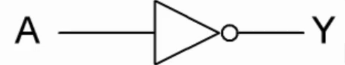
\includegraphics[scale=0.5]{01-porta_NOT.png}
	\caption{Porta NOT | Equação $Y = \overline{A}$}
\end{figure}

\begin{figure}[H]
	\centering
	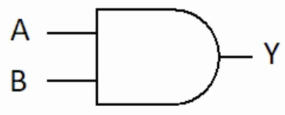
\includegraphics[scale=0.5]{02-porta_AND.png}
	\caption{Porta AND | Equação $Y = A\ . \ B $}
\end{figure}

\begin{figure}[H]
	\centering
	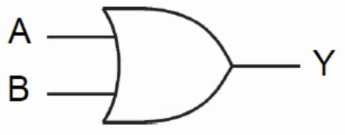
\includegraphics[scale=0.5]{03-porta_OR.png}
	\caption{Porta OR  | Equação $Y = A + B $}
\end{figure}

\subsubsection{Operadores Compostos}

\begin{figure}[H]
	\centering
	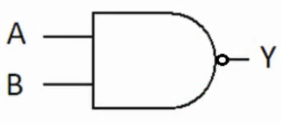
\includegraphics[scale=0.5]{04-porta_NAND.png}
	\caption{Porta OR  | Equação $Y = \overline{A\ . \ B} $}
\end{figure}

\begin{figure}[H]
	\centering
	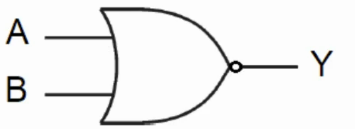
\includegraphics[scale=0.5]{05-porta_NOR.png}
	\caption{Porta OR  | Equação $Y = \overline{A + B} $}
\end{figure}

\begin{figure}[H]
	\centering
	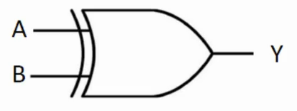
\includegraphics[scale=0.5]{06-porta_XOR.png}
	\caption{Porta OR  | Equação $Y = A \oplus B $}
\end{figure}

\subsubsection{Expressões Lógicas e Circuitos}

Podemos usar os operadores lógicos para criar expressões do tipo $ Y = (A+B).C $ que pode ser lida como "Y é igual a A ou B e C"\footnote{Usando os símbolos lógicos mais clássicos, podemos escrever como $Y: (A \lor B) \land C $}. Podemos também usar os diagramas de circuitos para representar exatamente essa mesma opração lógica.

\begin{figure}[H]
	\centering
	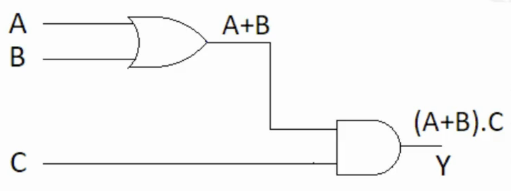
\includegraphics[scale=0.8]{07-operacao_logica.png}
\end{figure}


\subsection{Circuitos Lógicos Digitais Básicos}
\subsection{Introdução à Organização de Computadores}
\subsection{Unidade Central de Processamento - UCP}
\subsection{Memória}
\subsection{Entrada e Saída}

\section{Arquitetura de Computadores}
\subsection{Arquiteturas RISC e CISC}
\subsection{Arquitetura do Conjunto de Instruções: Exemplo do MIPS}
\subsection{Linguagem de Montagem}
\subsection{Conceito de Pipeline de Instruções}
\subsection{Paralelismo em Nível de Instruções}
\subsection{Paralelismo em Nível de Processadores}

%%%%%%%%%%%%%%%%%%%%%%%%%%%%%%%%%%%%%%%%%%%%%%%%%%%%%%%%%%%%%%%%%%%%%%%%
\chapter{Pensamento Computacional}
%%%%%%%%%%%%%%%%%%%%%%%%%%%%%%%%%%%%%%%%%%%%%%%%%%%%%%%%%%%%%%%%%%%%%%%%

\section{Bibliografia}

Bibliografia Básica

\begin{itemize}
	\item BEECHER, Karl. Computational Thinking - A beginner's guide to problem-solving and programming. Swindon, UK: BCS Learning \& Development Limited, 2017. (O´Reilly) EPUB ISBN-13: 978-1-78017-36-65
	\item FORBELLONE, André Luiz Villar; EBERSPACHER, Henri Frederico. Lógica de programação: a construção de algoritmos e estruturas de dados. 3. ed. São Paulo: Prentice Hall, 2005. xii, 218 p. ISBN 8576050242
	\item MANZANO, José Augusto N. G; OLIVEIRA, Jayr Figueiredo de. Algoritmos: lógica para desenvolvimento de programação de computadores. 28. ed. rev. e atual. São Paulo, SP: Érica, 2016. ISBN 9788536518657
\end{itemize}

Bibliografia Complementar

\begin{itemize}
	\item GUEDES, Sérgio (Org). Lógica de programação algorítmica. São Paulo: Pearson, 2014. ISBN 9788543005546
	\item MANZANO, José Augusto N. G. Estudo dirigido de algoritmos. 15. São Paulo Erica 2011 1 recurso online ISBN 9788536519067
	\item SOUZA, Marcos Fernando Ferreira de. Computadores e sociedade: da filosofia às linguagens de programação. Editora Intersaberes 208 ISBN 9788559722116
	\item TORRES, Fernando E. et al. Pensamento computacional. Porto Alegre: SAGAH, 2019. ISBN 978-85-9502-997-2
	\item FORBELLONE, André Luiz Villar; EBERSPACHER, Henri Frederico. Lógica de programação: a construção de algoritmos e estruturas de dados. 3. ed. São Paulo: Prentice Hall, 2005. xii, 218 p. ISBN 8576050242
\end{itemize}

\section{Conceitos e Competências de Pensamento Computacional}
\subsection{O que é?}
\subsection{A Importância do Pensamento Computacional}
\subsection{Visão Geral}
\subsection{Decomposição}
\subsection{Reconhecimento de Padrões}
\subsection{Abstração}
\subsection{Automação}
\subsection{Paralelização}
\subsection{Simulação}
\subsection{Avaliação de Soluções}

\section{Computação Desplugada}
\subsection{O que é?}
\subsection{A importância da Computação Desplugada}
\subsection{Compreensão de Texto}
\subsection{Adivinhação de Número}
\subsection{Roteiro Turístico}
\subsection{Nonograma}

%%%%%%%%%%%%%%%%%%%%%%%%%%%%%%%%%%%%%%%%%%%%%%%%%%%%%%%%%%%%%%%%%%%%%%%%
\part{Análise e Projeto de Software}
%%%%%%%%%%%%%%%%%%%%%%%%%%%%%%%%%%%%%%%%%%%%%%%%%%%%%%%%%%%%%%%%%%%%%%%%

%%%%%%%%%%%%%%%%%%%%%%%%%%%%%%%%%%%%%%%%%%%%%%%%%%%%%%%%%%%%%%%%%%%%%%%%
\chapter{Projeto: Desenvolvimento de uma Aplicação Interativa}
%%%%%%%%%%%%%%%%%%%%%%%%%%%%%%%%%%%%%%%%%%%%%%%%%%%%%%%%%%%%%%%%%%%%%%%%

%%%%%%%%%%%%%%%%%%%%%%%%%%%%%%%%%%%%%%%%%%%%%%%%%%%%%%%%%%%%%%%%%%%%%%%%
\chapter{Algoritmos e Estrutura de Dados}
%%%%%%%%%%%%%%%%%%%%%%%%%%%%%%%%%%%%%%%%%%%%%%%%%%%%%%%%%%%%%%%%%%%%%%%%

%%%%%%%%%%%%%%%%%%%%%%%%%%%%%%%%%%%%%%%%%%%%%%%%%%%%%%%%%%%%%%%%%%%%%%%%
\chapter{Desenvolvimento Web Back-End}
%%%%%%%%%%%%%%%%%%%%%%%%%%%%%%%%%%%%%%%%%%%%%%%%%%%%%%%%%%%%%%%%%%%%%%%%

%%%%%%%%%%%%%%%%%%%%%%%%%%%%%%%%%%%%%%%%%%%%%%%%%%%%%%%%%%%%%%%%%%%%%%%%
\chapter{Design de Interação}
%%%%%%%%%%%%%%%%%%%%%%%%%%%%%%%%%%%%%%%%%%%%%%%%%%%%%%%%%%%%%%%%%%%%%%%%

%%%%%%%%%%%%%%%%%%%%%%%%%%%%%%%%%%%%%%%%%%%%%%%%%%%%%%%%%%%%%%%%%%%%%%%%
\chapter{Engenharia de Requisitos de Software}
%%%%%%%%%%%%%%%%%%%%%%%%%%%%%%%%%%%%%%%%%%%%%%%%%%%%%%%%%%%%%%%%%%%%%%%%

%%%%%%%%%%%%%%%%%%%%%%%%%%%%%%%%%%%%%%%%%%%%%%%%%%%%%%%%%%%%%%%%%%%%%%%%
\chapter{Fundamentos de Redes de Computadores}
%%%%%%%%%%%%%%%%%%%%%%%%%%%%%%%%%%%%%%%%%%%%%%%%%%%%%%%%%%%%%%%%%%%%%%%%

%%%%%%%%%%%%%%%%%%%%%%%%%%%%%%%%%%%%%%%%%%%%%%%%%%%%%%%%%%%%%%%%%%%%%%%%
\chapter{Manipulação de Dados com SQL}
%%%%%%%%%%%%%%%%%%%%%%%%%%%%%%%%%%%%%%%%%%%%%%%%%%%%%%%%%%%%%%%%%%%%%%%%

%%%%%%%%%%%%%%%%%%%%%%%%%%%%%%%%%%%%%%%%%%%%%%%%%%%%%%%%%%%%%%%%%%%%%%%%
\chapter{Modelagem de Dados}
%%%%%%%%%%%%%%%%%%%%%%%%%%%%%%%%%%%%%%%%%%%%%%%%%%%%%%%%%%%%%%%%%%%%%%%%

%%%%%%%%%%%%%%%%%%%%%%%%%%%%%%%%%%%%%%%%%%%%%%%%%%%%%%%%%%%%%%%%%%%%%%%%
\chapter{Programação Modular}
%%%%%%%%%%%%%%%%%%%%%%%%%%%%%%%%%%%%%%%%%%%%%%%%%%%%%%%%%%%%%%%%%%%%%%%%

%%%%%%%%%%%%%%%%%%%%%%%%%%%%%%%%%%%%%%%%%%%%%%%%%%%%%%%%%%%%%%%%%%%%%%%%
\part{Processo de Negócio e Desenvolvimento de Software}
%%%%%%%%%%%%%%%%%%%%%%%%%%%%%%%%%%%%%%%%%%%%%%%%%%%%%%%%%%%%%%%%%%%%%%%%

%%%%%%%%%%%%%%%%%%%%%%%%%%%%%%%%%%%%%%%%%%%%%%%%%%%%%%%%%%%%%%%%%%%%%%%%
\chapter{Projeto: Desenvolvimento de uma Aplicação Móvel em um Ambiente de Negócio}
%%%%%%%%%%%%%%%%%%%%%%%%%%%%%%%%%%%%%%%%%%%%%%%%%%%%%%%%%%%%%%%%%%%%%%%%

%%%%%%%%%%%%%%%%%%%%%%%%%%%%%%%%%%%%%%%%%%%%%%%%%%%%%%%%%%%%%%%%%%%%%%%%
\chapter{Desenvolvimento de Aplicações Móveis}
%%%%%%%%%%%%%%%%%%%%%%%%%%%%%%%%%%%%%%%%%%%%%%%%%%%%%%%%%%%%%%%%%%%%%%%%

%%%%%%%%%%%%%%%%%%%%%%%%%%%%%%%%%%%%%%%%%%%%%%%%%%%%%%%%%%%%%%%%%%%%%%%%
\chapter{Estatística Descritiva}
%%%%%%%%%%%%%%%%%%%%%%%%%%%%%%%%%%%%%%%%%%%%%%%%%%%%%%%%%%%%%%%%%%%%%%%%

%%%%%%%%%%%%%%%%%%%%%%%%%%%%%%%%%%%%%%%%%%%%%%%%%%%%%%%%%%%%%%%%%%%%%%%%
\chapter{Gerência de Configuração}
%%%%%%%%%%%%%%%%%%%%%%%%%%%%%%%%%%%%%%%%%%%%%%%%%%%%%%%%%%%%%%%%%%%%%%%%

%%%%%%%%%%%%%%%%%%%%%%%%%%%%%%%%%%%%%%%%%%%%%%%%%%%%%%%%%%%%%%%%%%%%%%%%
\chapter{Gerência de Projetos de TI}
%%%%%%%%%%%%%%%%%%%%%%%%%%%%%%%%%%%%%%%%%%%%%%%%%%%%%%%%%%%%%%%%%%%%%%%%

%%%%%%%%%%%%%%%%%%%%%%%%%%%%%%%%%%%%%%%%%%%%%%%%%%%%%%%%%%%%%%%%%%%%%%%%
\chapter{Gerência de Requisitos de Software}
%%%%%%%%%%%%%%%%%%%%%%%%%%%%%%%%%%%%%%%%%%%%%%%%%%%%%%%%%%%%%%%%%%%%%%%%

%%%%%%%%%%%%%%%%%%%%%%%%%%%%%%%%%%%%%%%%%%%%%%%%%%%%%%%%%%%%%%%%%%%%%%%%
\chapter{Qualidade de Processos de Software}
%%%%%%%%%%%%%%%%%%%%%%%%%%%%%%%%%%%%%%%%%%%%%%%%%%%%%%%%%%%%%%%%%%%%%%%%

%%%%%%%%%%%%%%%%%%%%%%%%%%%%%%%%%%%%%%%%%%%%%%%%%%%%%%%%%%%%%%%%%%%%%%%%
\part{Infraestrutura para Sistemas de Software}
%%%%%%%%%%%%%%%%%%%%%%%%%%%%%%%%%%%%%%%%%%%%%%%%%%%%%%%%%%%%%%%%%%%%%%%%

%%%%%%%%%%%%%%%%%%%%%%%%%%%%%%%%%%%%%%%%%%%%%%%%%%%%%%%%%%%%%%%%%%%%%%%%
\chapter{Projeto: Desenvolvimento de um Aplicação Distribuída}
%%%%%%%%%%%%%%%%%%%%%%%%%%%%%%%%%%%%%%%%%%%%%%%%%%%%%%%%%%%%%%%%%%%%%%%%

%%%%%%%%%%%%%%%%%%%%%%%%%%%%%%%%%%%%%%%%%%%%%%%%%%%%%%%%%%%%%%%%%%%%%%%%
\chapter{APIs e Web Services}
%%%%%%%%%%%%%%%%%%%%%%%%%%%%%%%%%%%%%%%%%%%%%%%%%%%%%%%%%%%%%%%%%%%%%%%%

%%%%%%%%%%%%%%%%%%%%%%%%%%%%%%%%%%%%%%%%%%%%%%%%%%%%%%%%%%%%%%%%%%%%%%%%
\chapter{Arquitetura de Software Distribuído}
%%%%%%%%%%%%%%%%%%%%%%%%%%%%%%%%%%%%%%%%%%%%%%%%%%%%%%%%%%%%%%%%%%%%%%%%

%%%%%%%%%%%%%%%%%%%%%%%%%%%%%%%%%%%%%%%%%%%%%%%%%%%%%%%%%%%%%%%%%%%%%%%%
\chapter{Banco de Dados NoSQL}
%%%%%%%%%%%%%%%%%%%%%%%%%%%%%%%%%%%%%%%%%%%%%%%%%%%%%%%%%%%%%%%%%%%%%%%%

%%%%%%%%%%%%%%%%%%%%%%%%%%%%%%%%%%%%%%%%%%%%%%%%%%%%%%%%%%%%%%%%%%%%%%%%
\chapter{Cloud Computing}
%%%%%%%%%%%%%%%%%%%%%%%%%%%%%%%%%%%%%%%%%%%%%%%%%%%%%%%%%%%%%%%%%%%%%%%%

%%%%%%%%%%%%%%%%%%%%%%%%%%%%%%%%%%%%%%%%%%%%%%%%%%%%%%%%%%%%%%%%%%%%%%%%
\chapter{Projeto de Software}
%%%%%%%%%%%%%%%%%%%%%%%%%%%%%%%%%%%%%%%%%%%%%%%%%%%%%%%%%%%%%%%%%%%%%%%%

%%%%%%%%%%%%%%%%%%%%%%%%%%%%%%%%%%%%%%%%%%%%%%%%%%%%%%%%%%%%%%%%%%%%%%%%
\chapter{Teste de Software}
%%%%%%%%%%%%%%%%%%%%%%%%%%%%%%%%%%%%%%%%%%%%%%%%%%%%%%%%%%%%%%%%%%%%%%%%

%%%%%%%%%%%%%%%%%%%%%%%%%%%%%%%%%%%%%%%%%%%%%%%%%%%%%%%%%%%%%%%%%%%%%%%%
\part{Empreendedorismo e Inovação com Sistemas de Software}
%%%%%%%%%%%%%%%%%%%%%%%%%%%%%%%%%%%%%%%%%%%%%%%%%%%%%%%%%%%%%%%%%%%%%%%%

%%%%%%%%%%%%%%%%%%%%%%%%%%%%%%%%%%%%%%%%%%%%%%%%%%%%%%%%%%%%%%%%%%%%%%%%
\chapter{Projeto: Desenvolvimento de um Sistema Sociotecnológico Inovador}
%%%%%%%%%%%%%%%%%%%%%%%%%%%%%%%%%%%%%%%%%%%%%%%%%%%%%%%%%%%%%%%%%%%%%%%%

%%%%%%%%%%%%%%%%%%%%%%%%%%%%%%%%%%%%%%%%%%%%%%%%%%%%%%%%%%%%%%%%%%%%%%%%
\chapter{Complience em TI}
%%%%%%%%%%%%%%%%%%%%%%%%%%%%%%%%%%%%%%%%%%%%%%%%%%%%%%%%%%%%%%%%%%%%%%%%

%%%%%%%%%%%%%%%%%%%%%%%%%%%%%%%%%%%%%%%%%%%%%%%%%%%%%%%%%%%%%%%%%%%%%%%%
\chapter{Computadores e Sociedade}
%%%%%%%%%%%%%%%%%%%%%%%%%%%%%%%%%%%%%%%%%%%%%%%%%%%%%%%%%%%%%%%%%%%%%%%%

%%%%%%%%%%%%%%%%%%%%%%%%%%%%%%%%%%%%%%%%%%%%%%%%%%%%%%%%%%%%%%%%%%%%%%%%
\chapter{Empreendedorismo e Inovação}
%%%%%%%%%%%%%%%%%%%%%%%%%%%%%%%%%%%%%%%%%%%%%%%%%%%%%%%%%%%%%%%%%%%%%%%%

%%%%%%%%%%%%%%%%%%%%%%%%%%%%%%%%%%%%%%%%%%%%%%%%%%%%%%%%%%%%%%%%%%%%%%%%
\chapter{Implantação de Soluções de TI}
%%%%%%%%%%%%%%%%%%%%%%%%%%%%%%%%%%%%%%%%%%%%%%%%%%%%%%%%%%%%%%%%%%%%%%%%

%%%%%%%%%%%%%%%%%%%%%%%%%%%%%%%%%%%%%%%%%%%%%%%%%%%%%%%%%%%%%%%%%%%%%%%%
\chapter{Segurança Aplicada ao Desenvolvimento de Software}
%%%%%%%%%%%%%%%%%%%%%%%%%%%%%%%%%%%%%%%%%%%%%%%%%%%%%%%%%%%%%%%%%%%%%%%%

\end{document}
